\section{Funkce a jejich základní vlastnosti}
\begin{definition}
  \textbf{Funkcí} $f$ nazýváme každé zobrazení z $\mathbb R$ do $\mathbb R$.
\end{definition}

\begin{pozn}
  Obecněji by se funkce dala definovat také jako zobrazení z $\mathbb C$ do $\mathbb C$.
\end{pozn}

\begin{definition}
  Nechť $f\subseteq \mathbb R \times \mathbb R$ je funkce. Množinu
  \[
    D(f) = \left  \{ x \in \mathbb R:\exists ! y \in \mathbb R:y=f(x) \right \}
  \]
  nazveme \textbf{definičním oborem} funkce $f$. Množinu
  \[
    H(f) = \left  \{ y \in \mathbb R:\exists  x \in \mathbb R:y=f(x) \right \}
  \]
  nazveme \textbf{oborem hodnot} funkce $f$.
\end{definition}

\begin{priklad}
Určete definiční obor a obor hodnot funkce $y=x^2+x+1.$
\end{priklad}

\begin{reseni}
Definiční obor je $\mathbb R$, obor hodnot (množinu všech vyhovujících $a$)
získáme řešením rovnice $a=x^2+x+1$ v proměnné $x$:
\begin{align*}
	a &= x^2+x+1 \\
	0 &= x^2+x+1-a \\
	D&= 1-4(1-a)=4a-3.
\end{align*}
Aby rovnice měla řešení, musí být $D\geq 0$, tedy $4a-3\geq 0$, odkud dostáváme $a\geq 3/4$,
obor hodnot je tedy $\left < 3/4, \infty \right ). $
\end{reseni}

\begin{pozn}
  \textbf{Grafem funkce} rozumíme množinu všech bodů $[x,f(x)]$, kde $x\in D(f).$
\end{pozn}

\begin{priklad}
Nakreslete graf funkce $y=2-|x+1|.$
\end{priklad}

\begin{reseni}
	Graf této funkce (lomená přímka) bude mít zlomy jen tam, kde má zlomy absolutní hodnota,
	tj. v jejích nulových bodech. V tomto případě je to v bodě $x=-1$
	(protože pak $x+1=0$, kde se mění znaménko). Stačí tedy určit funkční hodnotu v tomto bodě
	a~v~libovolných dvou bodech nalevo a napravo od něj.
	\begin{figure}[ht!]
        \begin{center}
        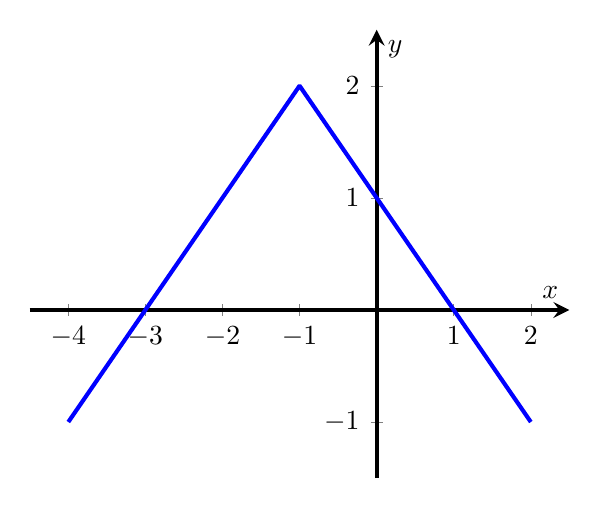
\begin{tikzpicture}
        \begin{axis}[
            axis lines = middle,
            xlabel = \(x\),
            ylabel = {\(y\)},
            xmin=-4.5,
            xmax=2.5,
            ymin=-1.5,
            ymax=2.5,
            line width=1.5pt,
        ]
        %Below the red parabola is defined
        \addplot [
            domain=-4:2,
            samples=500,
            color=blue,
        ]
        {2-abs(x+1)};

        \end{axis}
        \end{tikzpicture}
        \caption*{Graf $2- |x+1|$}
        \end{center}
        \end{figure}
\end{reseni}

\begin{priklad}
Nakreslete graf funkce $y=-2x^2+x-1$.
\end{priklad}

\begin{reseni}
Doplněním na čtverec získáme:
$$
	-2x^2+x-1 = -2 \left( x^2-\frac{1}{2}x+\frac{1}{2} \right ) = -2 \underbrace{\left( x-\frac{1}{4} \right )^2}_{x-\frac{1}{2}x+\frac{1}{16}} -2\left(-\frac{1}{16}+\frac{1}{2}\right)=-2 \left( x- \frac{1}{4} \right )^2-\frac{7}{8},
$$
odkud vidíme, že parabola je rozevřená dolů, je posunutá o $1/4$ doprava a o $7/8$ dolů.
\begin{figure}[ht!]
       \begin{center}
       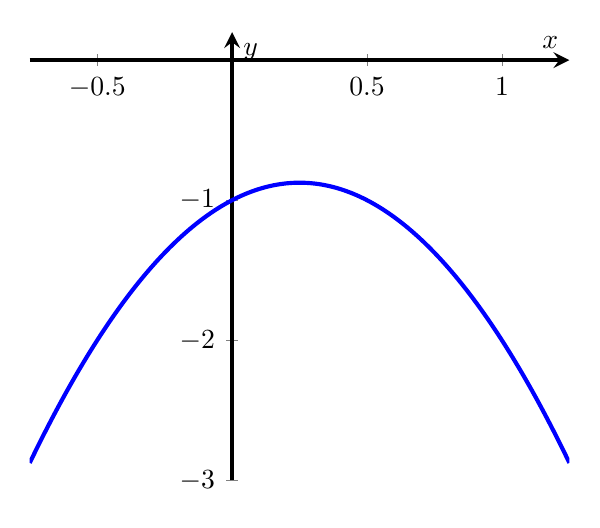
\begin{tikzpicture}
       \begin{axis}[
           axis lines = middle,
           xlabel = \(x\),
           ylabel = {\(y\)},
           xmin=-0.75,
           xmax=1.25,
           ymin=-3,
           ymax=0.2,
           line width=1.5pt,
       ]
       %Below the red parabola is defined
       \addplot [
           domain=-0.75:1.25,
           samples=500,
           color=blue,
       ]
       {-2*x*x+x-1};

       \end{axis}
       \end{tikzpicture}
       \caption*{Graf $-2x^2+x-1$}
       \end{center}
       \end{figure}
\end{reseni}

\begin{definition}\label{lichasuda}
  Funkce $f$ se nazývá \textbf{lichá} (resp. \textbf{sudá}), jestliže platí
  \begin{enumerate}[$i.$]
    \item $\forall x \in D(f): -x \in D(f)$ a
  	\item $\forall x \in D(f): f(-x)=-f(x)$, resp. $f(-x)=f(x)$.
  \end{enumerate}
\end{definition}

\begin{pozn}
  Graf liché funkce je souměrný podle počátku, graf sudé funkce je souměrný podle souřadné osy $y$.
\end{pozn}

\begin{priklad}
Určete paritu funkce $y=x^2$.
\end{priklad}

\begin{reseni}
Ověříme obě podmínky z definice \ref{lichasuda}:
\begin{enumerate}[$i.$]
\item $D(f)=\mathbb R$ -- platí,
\item $f(-x)=(-x)^2=x^2=f(x)$ -- platí, tedy funkce je sudá.
\end{enumerate}
\end{reseni}

\begin{definition}
  Funkce $f$ se nazývá \textbf{prostá}, právě tehdy když
  \[
    \forall x_1,x_2\in D(f): x_1\ne x_2 \implies f(x_1)\ne f(x_2).
  \]
\end{definition}

\begin{definition}
  Nechť $f$ je funkce a $M$ alespoň dvouprvková množina z $D(f)$. Řekneme, že funkce $f$ je na množině $M$
  \begin{enumerate}[$i.$]
    \item \textbf{rostoucí} $\iff \forall x_1, x_2 \in M: x_1 < x_2 \implies f(x_1) < f(x_2),$
    \item \textbf{klesající} $\iff \forall x_1, x_2 \in M: x_1 < x_2 \implies f(x_1) > f(x_2),$
    \item \textbf{neklesající} $\iff \forall x_1, x_2 \in M: x_1 < x_2 \implies f(x_1) \leq f(x_2),$
    \item \textbf{nerostoucí} $\iff \forall x_1, x_2 \in M: x_1 < x_2 \implies f(x_1) \geq f(x_2).$
  \end{enumerate}
  Je-li $f$ neklesající nebo nerostoucí, je \textbf{monotónní}. Pokud je klesající nebo rostoucí, je \textbf{ryze monotónní}.
\end{definition}

\begin{priklad}
Určete monotónnost funkce $y=x^2$ na množině $\mathbb R_0^+.$
\end{priklad}
\begin{reseni}
Je-li $x_1,x_2 >0$, pak $x_1 < x_2 \implies x_1^2 < x_1x_2.$ Obdobně $x_1x_2<x_2^2$.
Celkem tedy $x_1^2<x_2^2 \implies f(x_1)<f(x_2),$ tedy $f$ je rostoucí v $\mathbb R_0^+.$
\end{reseni}

\begin{definition}
  Nechť $f$ je funkce, $M\subseteq D(f)$. Řekneme, že funkce $f$ je na množině $M$
  \begin{enumerate}[$i.$]
    \item \textbf{shora omezená} $\iff \exists k \in \mathbb R: \forall x \in M: f(x)\leq k,$
    \item \textbf{zdola omezená} $\iff \exists k \in \mathbb R: \forall x \in M: f(x)\geq k,$
    \item \textbf{omezená} $\iff $ je zdola i shora omezená.
  \end{enumerate}
\end{definition}

\begin{definition}
  Nechť $f$ je funkce, $M \subseteq D(f)$, v ní prvek $a \in M$.
  Řekneme, že funkce $f$ má v~bodě $a$:
  \begin{enumerate}[$i.$]
    \item \textbf{ostré maximum} na množině $M$ právě tehdy, když $\forall x \in M\smallsetminus \left \{ a \right \}  : f(x) < f(a)$,
    \item \textbf{maximum} (neostré) na množině $M$ právě tehdy, když $\forall x \in M \smallsetminus \left \{ a \right \}: f(x) \leq f(a)$,
    \item \textbf{ostré minimum} na množině $M$ právě tehdy, když $\forall x \in M\smallsetminus \left \{ a \right \}: f(x) > f(a)$,
    \item \textbf{minimum} (neostré) na množině $M$ právě tehdy, když $\forall x \in M\smallsetminus \left \{ a \right \} : f(x) \geq f(a)$.
  \end{enumerate}
\end{definition}

\begin{definition}
  Nechť $f$ je funkce. Funkce $f$ se nazývá \textbf{periodická}, pokud $\exists p \in \mathbb R^{+}: \forall x \in D(f):$
  \begin{enumerate}
    \item $x \in D(f) \implies x \pm p \in D(f)$ a
    \item $f(x) = f(x \pm p)$.
  \end{enumerate}
  Číslo $p$ se nazývá \textbf{periodou} této funkce. Periodu $p_0$ nazveme \textbf{nejmenší periodou} funkce, pokud pro všechny ostatní periody $p$ platí $p > p_0$. V opačném případě se funkce nazývá \textbf{neperiodická}.
\end{definition}

\begin{definition}
  Nechť máme funkci $f: y = f(u)$ s definičním oborem $D(f)$ a funkci $g: u=g(x)$ s oborem hodnot $H(g)$. Jestliže je $H(g) \subseteq D(f)$, pak funkci $h: y = f(g(x))$ nazveme \textbf{složenou funkcí} (někdy píšeme též $h=f \circ g$).
\end{definition}

\begin{definition}
  \textbf{Dirichletova funkce} je definována následovně:
  $$\mathbf{D} (x) = \begin{cases}
1, & \text{ je-li } x \in \mathbb Q, \\
0 & \text{ jinak}.
  \end{cases}  $$
\end{definition}

\begin{definition}
  Funkce \textbf{signum} je definována následovně: $$\operatorname {sgn} x={\begin{cases}-1,& \textrm{je-li }x<0,\\0,&\textrm{je-li }x=0,\\1,&\textrm{je-li }x>0.\end{cases}}$$
\end{definition}

\begin{definition}
  Nechť $x \in \mathbb{R}$ je libovolné číslo. Pak existuje právě jedna dvojice $z \in \mathbb{Z}, a \in \left \langle 0;1 \right) \text{ tak, že } x = z + a$.
Číslo $z$ nazýváme \textbf{celou částí} čísla $x$ a zapisujeme $[x] = z$, někdy taky $\lfloor x \rfloor = z$.
\end{definition}

\begin{pozn}
    Pro definici limity a funkce spojité viz kapitolu \ref{limita},
    dále definici derivace def. \ref{derivace}, funkce konvexní a
    konkávní def. \ref{konvkonk} a konečně definici integrálu def. \ref{integral}.
\end{pozn}
